\appendix

\section{Proof of Theorem~\ref{thm:monotonicity}}
\label{app:proof}

The replaced judge $J_K'$ is \emph{pivotal} exactly when $t{-}1$ of the remaining $K{-}1$ judges have already failed. Formally, let $S = \sum_{j=1}^{K-1} X_j^a$ denote the number of failures among the shared judges. The panel fails if and only if the $K$-th judge also fails when $S = t{-}1$, or when $S \geq t$ regardless of the $K$-th judge:
\begin{align}
\mathrm{ASR}(\mathcal{P}, a) &= \Pr(S \geq t) + \Pr(S = t{-}1) \cdot \Pr(X_K^a {=} 1 \mid S = t{-}1).
\end{align}
Since $\Pr(X_{K'}^a {=} 1 \mid \mathbf{X}_{-K}^a {=} \mathbf{x}_{-K}) \geq \Pr(X_K^a {=} 1 \mid \mathbf{X}_{-K}^a {=} \mathbf{x}_{-K})$ for all attacks $a$ and realizations $\mathbf{x}_{-K}$ (by hypothesis), the second term is weakly larger for $\mathcal{P}'$ than for $\mathcal{P}$ under every attack. Taking the supremum over attacks preserves the inequality: $\mathrm{ASR}^*(\mathcal{P}') \geq \mathrm{ASR}^*(\mathcal{P})$. The result holds under arbitrary inter-judge correlations and any attack space $\mathcal{A}$.

\section{Robustness Correction Methods}
\label{app:robustness_methods}

The 455 panels are constructed combinatorially from 15 shared judges: each judge appears in $\binom{14}{2} = 91$ panels, inducing correlated residuals across panel-level observations. Standard OLS assumes independent errors, potentially inflating significance. We apply three corrections.

\paragraph{Clustered Standard Errors.} Because each panel of $K{=}3$ judges does not map to a single cluster, we perform three separate one-way clusterings (one for each judge position in the ordered panel tuple) using CR1 bias-corrected sandwich estimators (13 clusters per position). The reported standard error for each coefficient is the maximum across the three clusterings, yielding the most conservative inference.

\paragraph{Mixed Effects.} For each of the three judge positions, we fit a linear mixed-effects model with a random intercept for the judge occupying that position, estimating $K_{\mathrm{eff}}$ and $\eta_{\max}$ as fixed effects. The reported $p$-value for each coefficient is the maximum across the three models.

\paragraph{Wild Cluster Bootstrap.} We perform $B{=}9{,}999$ bootstrap resamples using Rademacher weights, clustering by each of the three panel positions in turn and taking the maximum $p$-value across positions (the most conservative aggregation). This approach avoids distributional assumptions on the cluster structure.

\section{Extended Analysis}
\label{app:extended_analysis}

\subsection{BFT Reversal Mechanism: Detailed Evidence}
\label{app:bft_reversal}

Under standard OLS, the regression results (Table~\ref{tab:dominance}) show $\eta_{\max}$ significant in 10 of 12 conditions and $K_{\mathrm{eff}}$ positively associated with ASR in all 12. Non-independence correction attenuates both predictors: under wild cluster bootstrap, $\eta_{\max}$ retains 3/12 and $K_{\mathrm{eff}}$ retains 4/12, with $K_{\mathrm{eff}}$ slightly ahead. The directional pattern (all $K_{\mathrm{eff}}$ point estimates positive) persists uniformly. The random-fault contrast (\S\ref{sec:rf_contrast}) sharpens this: under random faults, $K_{\mathrm{eff}}$'s positive association with panel error survives all corrections (2/2 conditions, $R^2 = 0.73$--$0.81$), indicating a genuine relationship whose statistical confidence attenuates under adaptive attack (4/12 after correction).

\begin{figure}[h]
\centering
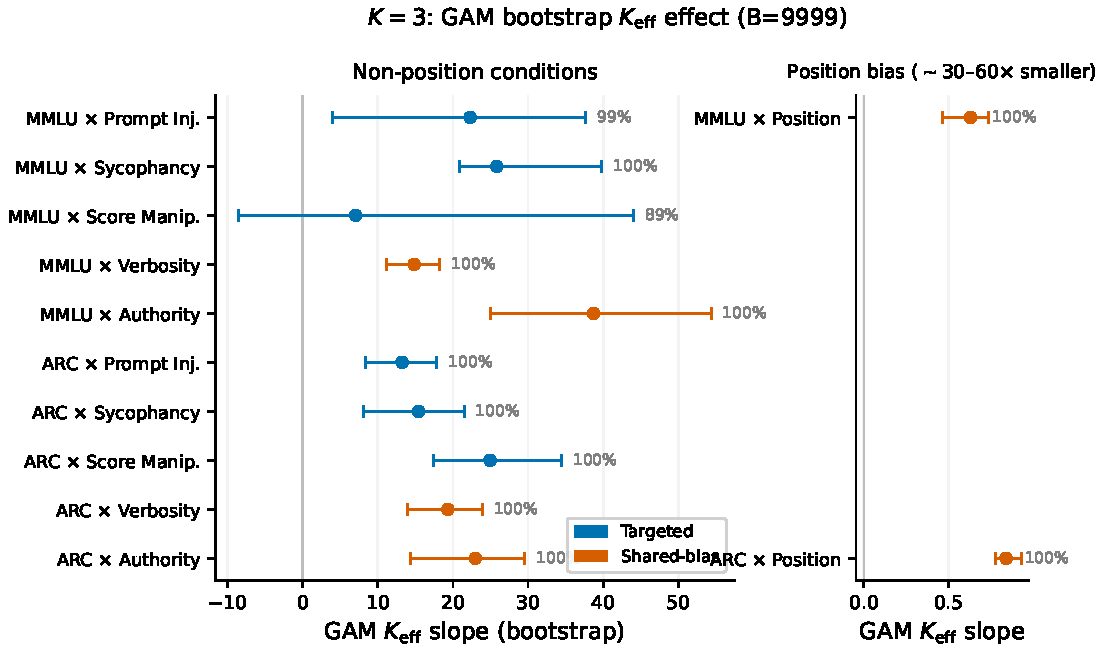
\includegraphics[width=\columnwidth]{figures/fig2_gam_keff_split.pdf}
\caption{GAM bootstrap $K_{\mathrm{eff}}$ effect direction at $K{=}3$ ($B{=}9999$). All 12 conditions show positive $K_{\mathrm{eff}}$ direction (88.9--100\% bootstrap rate). The Kruskal--Wallis test finds no significant magnitude difference between targeted and shared-bias attacks ($p{=}0.200$).}
\label{fig:gam_split}
\end{figure}

Under corrected data (V2), all 12 $K_{\mathrm{eff}}$ OLS coefficients are positive. The previously reported negative ARC $\times$ sycophancy coefficient ($\hat{\beta}_{\mathrm{std}} = -0.192$) was an artifact of error-as-tie handling; after correction, it becomes positive ($\hat{\beta}_{\mathrm{std}} = +0.257$). GAM bootstrap confirms the uniform positive direction: 12/12 conditions at $K{=}3$ (88.9--100\% positive rate) and 12/12 at $K{=}5$ (100\%).

\subsection{Diversity--Capability Tradeoff}
\label{app:diversity_capability}

The $r = 0.70$--$0.81$ correlation between $K_{\mathrm{eff}}$ and $\eta_{\max}$ ($K{=}3$ to $K{=}5$) reflects a structural feature of the current LLM ecosystem: maximizing panel diversity requires sampling across capability tiers, which systematically introduces less capable and therefore more vulnerable judges. The structural correlation is unaffected by SE correction; it is a property of the model ecosystem, not an artifact of panel overlap. However, the high confound combined with fragile independent significance means that observational regression cannot reliably disentangle diversity's causal contribution from the capability deficit that co-occurs with it.

\begin{figure}[h]
\centering
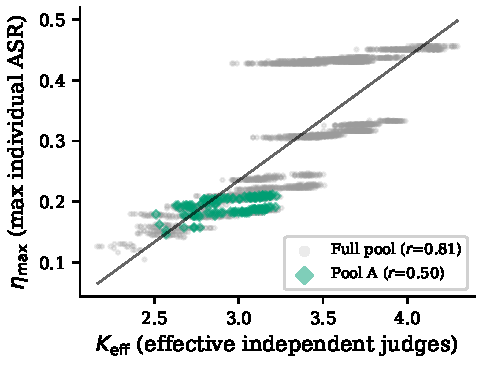
\includegraphics[width=\columnwidth]{figures/fig_keff_eta_scatter.pdf}
\caption{Panel-level correlation between $K_{\mathrm{eff}}$ and $\eta_{\max}$ at $K{=}5$ ($n{=}3{,}003$ panels). Full model pool (gray, $r{=}0.81$) exhibits strong collinearity; capability-matched Pool~A (orange diamonds, $r{=}0.50$, 126 panels) shows reduced confounding.}
\label{fig:keff_eta_scatter}
\end{figure}

Family-level labels provide indirect evidence that capability proximity matters more than taxonomic grouping: family membership is not a significant predictor of panel vulnerability ($p = 0.179$ on MMLU, $p = 0.385$ on ARC), consistent with models from the same provider exhibiting heterogeneous vulnerability profiles that vary by capability tier rather than by shared architecture \citep{kuncheva2003measures}.

\subsection{Aggregation Mechanism Details}
\label{app:aggregation_details}

Bayesian calibration attenuates $K_{\mathrm{eff}}$ significance (5+/1$-$) and reduces overall predictability ($R^2{=}0.087$), but $\eta_{\max}$ persists (9/12 under OLS), providing partial defense. The mechanism is calibrated reliability weighting: by estimating each judge's confusion matrix on clean data, Bayesian aggregation downweights weak judges, reducing the diversity channel while the individual weakness channel remains active. Threshold voting amplifies both channels because any single dissenting judge vetoes the panel decision, making compositional factors highly predictive of attack success ($R^2{=}0.829$). Bayesian calibration requires a clean accuracy prior, and an adaptive attacker aware of this calibration could target the prior itself \citep{tambe2011security}.

\begin{figure}[h]
\centering
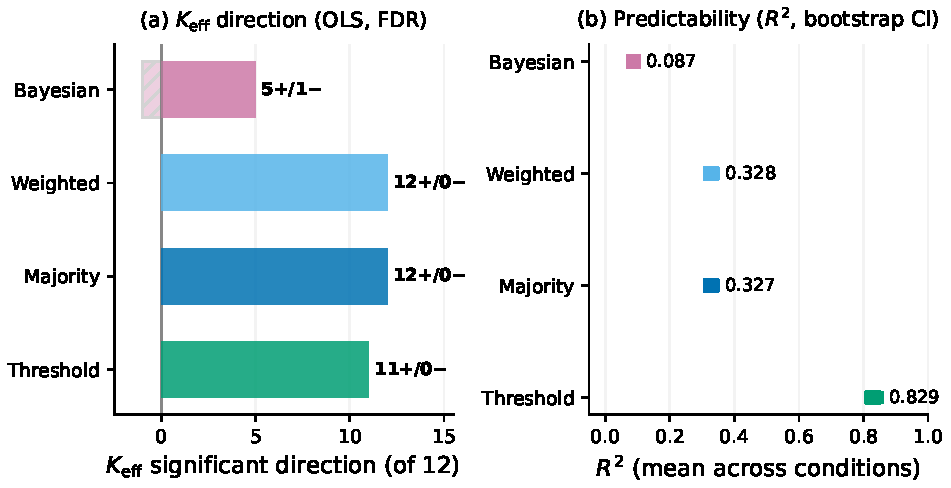
\includegraphics[width=\columnwidth]{figures/fig3_aggregation_gradient.pdf}
\caption{Distribution of $K_{\mathrm{eff}}$ coefficients across aggregation methods. Majority and weighted voting show uniformly positive $K_{\mathrm{eff}}$ direction (12+/0$-$). Bayesian calibration reduces overall predictability ($R^2{=}0.087$) with predominantly positive direction (5+/1$-$).}
\label{fig:aggregation}
\end{figure}

\subsection{Aggregation at \texorpdfstring{$K{=}5$}{K=5}}
\label{app:aggregation_k5}

Table~\ref{tab:aggregation_k5} extends the aggregation analysis to $K{=}5$ (3{,}003 panels) under wild cluster bootstrap with 5-position max-$p$. All four aggregation methods yield identical $K_{\mathrm{eff}}$ significance (7/12), with $\eta_{\max}$ uniformly low (2--3/12). The Bayesian attenuation observed at $K{=}3$ (5+/1$-$; Table~\ref{tab:aggregation}) does not persist: $K_{\mathrm{eff}}$ reaches 7/12 regardless of aggregation rule. Predictability still varies ($\bar{R}^2$: threshold 0.408, Bayesian 0.166), but the diversity channel operates uniformly across all methods. At $K{=}7$, however, methods diverge again: Bayesian neutralization returns (0/12) while threshold voting strengthens to 10/12 (Table~\ref{tab:aggregation_k7}).

\begin{table}[h]
\centering
\small
\begin{tabular}{lccc}
\toprule
\textbf{Aggregation} & $\boldsymbol{\eta_{\max}}$ \textbf{sig} & $\boldsymbol{K_{\mathrm{eff}}}$ \textbf{sig} & $\boldsymbol{\bar{R}^2}$ \\
\midrule
Majority   & 2/12  & 7/12 & 0.285 \\
Weighted   & 2/12  & 7/12 & 0.275 \\
Threshold  & 3/12  & 7/12 & 0.408 \\
Bayesian   & 2/12  & 7/12 & 0.166 \\
\bottomrule
\end{tabular}
\caption{Aggregation method comparison at $K{=}5$ (3{,}003 panels, wild cluster bootstrap with 5-position max-$p$, BH FDR $\alpha{=}0.05$). All four methods converge to $K_{\mathrm{eff}}$ 7/12, unlike the differentiated pattern at $K{=}3$ (Table~\ref{tab:aggregation}).}
\label{tab:aggregation_k5}
\end{table}

\subsection{Aggregation at \texorpdfstring{$K{=}7$}{K=7}}
\label{app:aggregation_k7}

Table~\ref{tab:aggregation_k7} extends the aggregation analysis to $K{=}7$ (6{,}435 panels) under wild cluster bootstrap with 7-position max-$p$. Unlike the uniform convergence at $K{=}5$ (all methods 7/12), aggregation methods diverge at $K{=}7$: threshold voting strengthens to 10/12 while Bayesian calibration drops to 0/12, restoring the neutralization pattern absent at $K{=}5$.

\begin{table}[h]
\centering
\small
\begin{tabular}{lccc}
\toprule
\textbf{Aggregation} & $\boldsymbol{\eta_{\max}}$ \textbf{sig} & $\boldsymbol{K_{\mathrm{eff}}}$ \textbf{sig} & $\boldsymbol{\bar{R}^2}$ \\
\midrule
Majority   & 1/12  & 8/12 & 0.244 \\
Weighted   & 1/12  & 6/12 & 0.207 \\
Threshold  & 8/12  & 10/12 & 0.509 \\
Bayesian   & 1/12  & 0/12 & 0.105 \\
\bottomrule
\end{tabular}
\caption{Aggregation method comparison at $K{=}7$ (6{,}435 panels, wild cluster bootstrap with 7-position max-$p$, BH FDR $\alpha{=}0.05$). Unlike $K{=}5$ where all methods converge to 7/12, $K{=}7$ shows method divergence: threshold voting reaches 10/12 while Bayesian calibration returns to full $K_{\mathrm{eff}}$ neutralization (0/12).}
\label{tab:aggregation_k7}
\end{table}

\subsection{Metric Robustness Under Partial Panel Information}
\label{app:oracle}

The main analysis computes $\eta_{\max}$ with full knowledge of panel composition (all three judges known). In deployment, a practitioner selecting or auditing a panel may know only a subset of the constituent judges. We test whether $\eta_{\max}$ retains predictive power under such partial information by recomputing it from two of the three panel members: for each panel, we cycle through all $\binom{3}{1} = 3$ leave-one-out masks, compute $\eta_{\max}$ from the two known judges, and average the regression estimates across masking scenarios.

Under the most conservative inference (partial information + clustered SE), $\eta_{\max}$ remains the sole significant predictor with $\hat{\beta}_{\mathrm{std}} = 0.589$, achieving significance in 12/12 conditions, stronger than the oracle baseline (4/12 under clustered SE). $K_{\mathrm{eff}}$ loses all predictive power (0/12). The averaging over masking scenarios smooths estimation noise inherent in the three-judge oracle computation, strengthening the $\eta_{\max}$ signal. This demonstrates that $\eta_{\max}$ computed from partial panel information is robust to incomplete composition knowledge and retains (indeed improves) its predictive power for panel ASR.

\section{Panel Selection Strategy Comparison}
\label{app:panel_selection}

\begin{figure}[h]
\centering
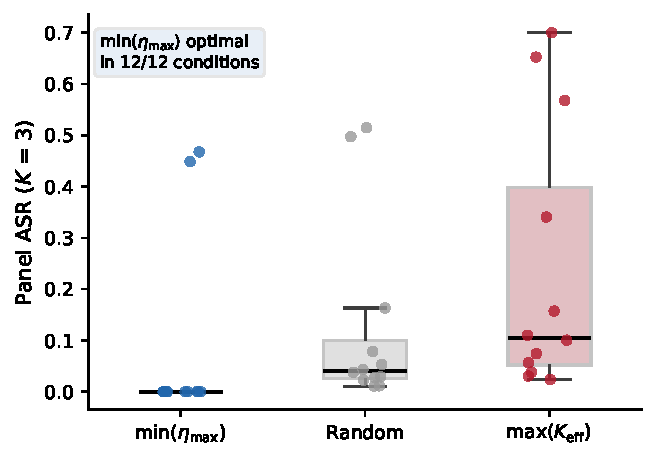
\includegraphics[width=\columnwidth]{figures/fig4_panel_design.pdf}
\caption{Panel attack success rate under three selection strategies. $\min(\eta_{\max})$ achieves lowest ASR in 12/12 conditions, confirming that robustness-first selection dominates diversity-maximizing strategies.}
\label{fig:panel_design}
\end{figure}

Figure~\ref{fig:panel_design} compares three panel selection strategies: $\min(\eta_{\max})$ (select the panel minimizing weakest-judge vulnerability), random selection, and $\max(K_{\mathrm{eff}})$ (maximize diversity). The $\min(\eta_{\max})$ strategy achieves the lowest ASR in all 12 conditions, consistent with the weakest-link dominance documented in \S\ref{sec:dominance}.

\section{Clustered Standard Error Analysis}
\label{app:forest_plot}

Under clustered standard errors (clustering on the $K$ judge positions), $\eta_{\max}$ retains significance in 4/12 conditions while $K_{\mathrm{eff}}$ achieves significance in 0/12. This contrasts with OLS ($\eta_{\max}$ 10/12, $K_{\mathrm{eff}}$ 12/12) and wild cluster bootstrap ($\eta_{\max}$ 3/12, $K_{\mathrm{eff}}$ 4/12), illustrating how the choice of inference method modulates apparent significance at $K{=}3$ while coefficient direction remains positive (12/12) for $K_{\mathrm{eff}}$ across all methods, with significance ranging from 0/12 to 12/12 (Figure~\ref{fig:robustness}).

\section{Robustness Checks: Subsampling and Specification}
\label{app:robustness_checks}

Table~\ref{tab:robustness_checks} summarizes regression results across model subsets and alternative specifications at $K{=}5$, testing whether the predictor shift is robust to collinearity reduction and specification choice.

\begin{table}[h]
\centering
\small
\begin{tabular}{lcccc}
\toprule
\textbf{Subset / Method} & $\boldsymbol{r}$ & $\boldsymbol{\eta_{\max}}$ & $\boldsymbol{K_{\mathrm{eff}}}$ & \textbf{Trans.} \\
\midrule
Full bootstrap       & 0.81 & 2/12 & 7/12 & \checkmark \\
API-only (9) clust.  & 0.85 & 8/12 & 3/12 & --- \\
Cap-matched A (5A+4L) & 0.50 & ---  & 9/12 & \checkmark\checkmark \\
Cap-matched B (6A+3L) & 0.73 & ---  & 2/12 & --- \\
Fractional logit     & 0.81 & 4/12 & 11/12 & \checkmark \\
\bottomrule
\end{tabular}
\caption{Predictor shift robustness at $K{=}5$ across model subsets and specifications. $r$: correlation between $K_{\mathrm{eff}}$ and $\eta_{\max}$. $\eta_{\max}$ and $K_{\mathrm{eff}}$ columns show FDR-significant counts out of 12 conditions. Trans.: whether $K_{\mathrm{eff}}$ dominates $\eta_{\max}$. API-only models ($r{=}0.85$, VIF${=}4.4$) show partially collinear predictors; capability-matched subsamples ($r{=}0.50$) strengthen the shift. Fractional logit \citep{papke1996econometric} confirms OLS patterns with 98.6\% directional agreement (71/72 direction matches; the single discordance is $\eta_{\max}$ at $K{=}7$ for ARC $\times$ score manipulation).}
\label{tab:robustness_checks}
\end{table}

The API-only subset ($r{=}0.85$, VIF${=}4.4$) demonstrates that elevated collinearity between $K_{\mathrm{eff}}$ and $\eta_{\max}$ partially inflates standard errors: both predictors achieve moderate significance but neither dominates, and the predictor shift does not replicate. Breaking collinearity through capability-matched subsampling (pool~A, $r{=}0.50$) strengthens $K_{\mathrm{eff}}$'s emergence to 9/12, comparable to the full-pool 7/12. Pool~B ($r{=}0.73$) falls near the decorrelation threshold, and the shift weakens accordingly. Random 9-model subsampling (1{,}000 trials) confirms an inverted-U: $K_{\mathrm{eff}}$ dominance rate peaks when the subsample includes 3--4 local models (maximizing capability spread) and drops when the pool is too homogeneous (Appendix~\ref{app:random_subsample}).

\section{Random Subsample Analysis}
\label{app:random_subsample}

To test whether the predictor shift depends on model pool composition, we randomly sample 9 of 15 models (1{,}000 trials), construct all $\binom{9}{5}$ panels, and run the bootstrap analysis at $K{=}5$. We stratify by the number of local models ($n_{\mathrm{local}} \in \{0, \ldots, 6\}$) in each subsample.

Under clustered standard errors, $K_{\mathrm{eff}}$ is the dominant predictor in 51.4\% of subsamples (mean significance 1.85/12), with an inverted-U as a function of $n_{\mathrm{local}}$: subsamples with 3--4 local models (maximizing capability range) achieve the highest $K_{\mathrm{eff}}$ significance rate, while all-API ($n_{\mathrm{local}}{=}0$) and heavily-local ($n_{\mathrm{local}}{\geq}5$) subsamples show reduced detection. Significance is attenuated relative to the full pool by smaller sample sizes (126 vs.\ 3{,}003 panels at $K{=}5$), but the shift direction holds in the majority of subsamples. This confirms that the shift's detectability depends on capability diversity in the model pool rather than pool size per se.

\section{Attacked $K_{\mathrm{eff}}$ Stability}
\label{app:attacked_keff}

$K_{\mathrm{eff}}$ is computed from clean (unattacked) pairwise MI (\S\ref{sec:experiments}), but used to predict vulnerability under attack. We verify this assumption by recomputing MI from judge outputs under each attack type and comparing clean vs.\ attacked $K_{\mathrm{eff}}$ via Spearman rank correlation across all panels.

\begin{table}[h]
\centering
\small
\begin{tabular}{lcc}
\toprule
\textbf{Attack} & \textbf{MMLU $\rho$} & \textbf{ARC $\rho$} \\
\midrule
Score manipulation & 0.98 & 0.99 \\
Authority bias     & 0.95 & 0.97 \\
Sycophancy         & 0.91 & 0.92 \\
Verbosity bias     & 0.91 & 0.92 \\
Prompt injection   & 0.63 & 0.60 \\
Position bias      & 0.60 & 0.08 \\
\bottomrule
\end{tabular}
\caption{Spearman rank correlation between clean and attacked $K_{\mathrm{eff}}$ across 455 panels ($K{=}3$). Four attack types preserve MI structure ($\rho{\geq}0.91$); prompt injection shows moderate perturbation ($\rho{\approx}0.60$--$0.63$); position bias substantially disrupts pairwise dependencies.}
\label{tab:attacked_keff}
\end{table}

Four attack types (score manipulation, authority bias, sycophancy, verbosity bias) preserve MI structure with $\rho{\geq}0.91$ on both benchmarks, validating the use of clean $K_{\mathrm{eff}}$ as a predictor. Prompt injection shows moderate perturbation ($\rho{\approx}0.60$--$0.63$), consistent with its mechanism of overriding evaluation instructions, which can alter pairwise agreement patterns. Position bias substantially disrupts MI structure ($\rho{=}0.08$ on ARC, $p{=}0.10$), consistent with its anomalous regression behavior in Table~\ref{tab:dominance} (sole non-significant $\eta_{\max}$ condition) and suggesting that positional reordering fundamentally changes inter-judge dependence rather than merely introducing noise.

\section{Cinelli--Hazlett Sensitivity Analysis}
\label{app:sensitivity}

We apply the Cinelli--Hazlett omitted variable bias framework to quantify how robust $K_{\mathrm{eff}}$'s coefficient is to unobserved confounders. For each of the 36 conditions ($3K \times 2$ benchmarks $\times$ $6$ attacks), we compute the robustness value (RV): the minimum strength an unobserved confounder must have, in terms of partial $R^2$ with both treatment and outcome, to reduce $K_{\mathrm{eff}}$'s coefficient to zero.

\begin{table}[h]
\centering
\footnotesize
\setlength{\tabcolsep}{3pt}
\begin{tabular}{rcllcccc}
\toprule
$\boldsymbol{K}$ & \textbf{Data} & \textbf{Attack} & \textbf{RV} & $\boldsymbol{\eta}$ $\boldsymbol{R^2_{\mathrm{tr}}}$ & $\boldsymbol{\eta}$ $\boldsymbol{R^2_{\mathrm{out}}}$ & \textbf{Exc.} \\
\midrule
3 & MMLU & Prompt inj.    & 0.419 & 0.587 & 0.059 & -- \\
3 & MMLU & Sycophancy     & 0.412 & 0.347 & 0.098 & \checkmark \\
3 & MMLU & Score manip.   & 0.410 & 0.735 & 0.002 & -- \\
3 & MMLU & Verbosity      & 0.330 & 0.342 & 0.203 & -- \\
3 & MMLU & Position bias  & 0.291 & 0.446 & 0.043 & -- \\
3 & MMLU & Authority bias & 0.371 & 0.493 & 0.019 & -- \\
3 & ARC  & Prompt inj.    & 0.303 & 0.654 & 0.028 & -- \\
3 & ARC  & Sycophancy     & 0.105 & 0.629 & 0.129 & -- \\
3 & ARC  & Score manip.   & 0.273 & 0.838 & 0.003 & -- \\
3 & ARC  & Verbosity      & 0.259 & 0.658 & 0.047 & -- \\
3 & ARC  & Position bias  & 0.265 & 0.850 & 0.001 & -- \\
3 & ARC  & Authority bias & 0.224 & 0.582 & 0.056 & -- \\
\addlinespace
5 & MMLU & Prompt inj.    & 0.455 & 0.379 & 0.176 & \checkmark \\
5 & MMLU & Sycophancy     & 0.303 & 0.106 & 0.135 & \checkmark \\
5 & MMLU & Score manip.   & 0.321 & 0.597 & 0.003 & -- \\
5 & MMLU & Verbosity      & 0.235 & 0.120 & 0.206 & \checkmark \\
5 & MMLU & Position bias  & 0.131 & 0.272 & 0.090 & -- \\
5 & MMLU & Authority bias & 0.064 & 0.277 & 0.031 & -- \\
5 & ARC  & Prompt inj.    & 0.318 & 0.696 & 0.001 & -- \\
5 & ARC  & Sycophancy     & 0.103 & 0.555 & 0.063 & -- \\
5 & ARC  & Score manip.   & 0.196 & 0.800 & ${<}0.001$ & -- \\
5 & ARC  & Verbosity      & 0.135 & 0.642 & 0.034 & -- \\
5 & ARC  & Position bias  & 0.400 & 0.778 & 0.040 & -- \\
5 & ARC  & Authority bias & 0.181 & 0.509 & 0.012 & -- \\
\addlinespace
7 & MMLU & Prompt inj.    & 0.522 & 0.289 & 0.126 & \checkmark \\
7 & MMLU & Sycophancy     & 0.301 & 0.077 & 0.078 & \checkmark \\
7 & MMLU & Score manip.   & 0.393 & 0.515 & 0.004 & -- \\
7 & MMLU & Verbosity      & 0.205 & 0.078 & 0.195 & \checkmark \\
7 & MMLU & Position bias  & 0.207 & 0.179 & 0.073 & \checkmark \\
7 & MMLU & Authority bias & 0.005 & 0.200 & 0.011 & -- \\
7 & ARC  & Prompt inj.    & 0.355 & 0.629 & 0.004 & -- \\
7 & ARC  & Sycophancy     & 0.117 & 0.535 & 0.065 & -- \\
7 & ARC  & Score manip.   & 0.165 & 0.717 & 0.001 & -- \\
7 & ARC  & Verbosity      & 0.165 & 0.599 & 0.028 & -- \\
7 & ARC  & Position bias  & 0.422 & 0.705 & 0.046 & -- \\
7 & ARC  & Authority bias & 0.179 & 0.514 & 0.003 & -- \\
\bottomrule
\end{tabular}
\caption{Cinelli--Hazlett sensitivity analysis for $K_{\mathrm{eff}}$'s coefficient across 36 conditions. RV: robustness value (minimum partial $R^2$ an unobserved confounder must have with both $K_{\mathrm{eff}}$ and ASR to nullify the coefficient). $\eta$ $R^2_{\mathrm{tr}}$/$R^2_{\mathrm{out}}$: partial $R^2$ of $\eta_{\max}$ with $K_{\mathrm{eff}}$ (treatment) and ASR (outcome). Exc.: \checkmark\ if RV exceeds $\eta_{\max}$'s partial $R^2$ with treatment, indicating $K_{\mathrm{eff}}$'s coefficient is robust to the known capability confound. RV exceeds $\eta_{\max}$ in 11/36 conditions ($K{=}3$: 4/12, $K{=}5$: 3/12, $K{=}7$: 4/12).}
\label{tab:sensitivity}
\end{table}

RV ranges from 0.005--0.59 across the 36 conditions (median by $K$: 0.30 at $K{=}3$, 0.22 at $K{=}5$, 0.21 at $K{=}7$), revealing heterogeneous robustness: some conditions show $K_{\mathrm{eff}}$ coefficients robust to strong confounders (e.g., $K{=}7$ MMLU prompt injection, RV${=}0.52$), while others are fragile (e.g., $K{=}7$ MMLU authority bias, RV${=}0.005$). The known $\eta_{\max}$ confound exceeds RV in 25/36 conditions ($K{=}3$: 8/12, $K{=}5$: 9/12, $K{=}7$: 8/12). RV exceeds $\eta_{\max}$ in 3--4/12 conditions across all $K$ values (4/12 at $K{=}3$, 3/12 at $K{=}5$, 4/12 at $K{=}7$), indicating that $K_{\mathrm{eff}}$'s robustness to omitted variable bias is stable rather than monotonically increasing with panel size.

\begin{figure}[h]
\centering
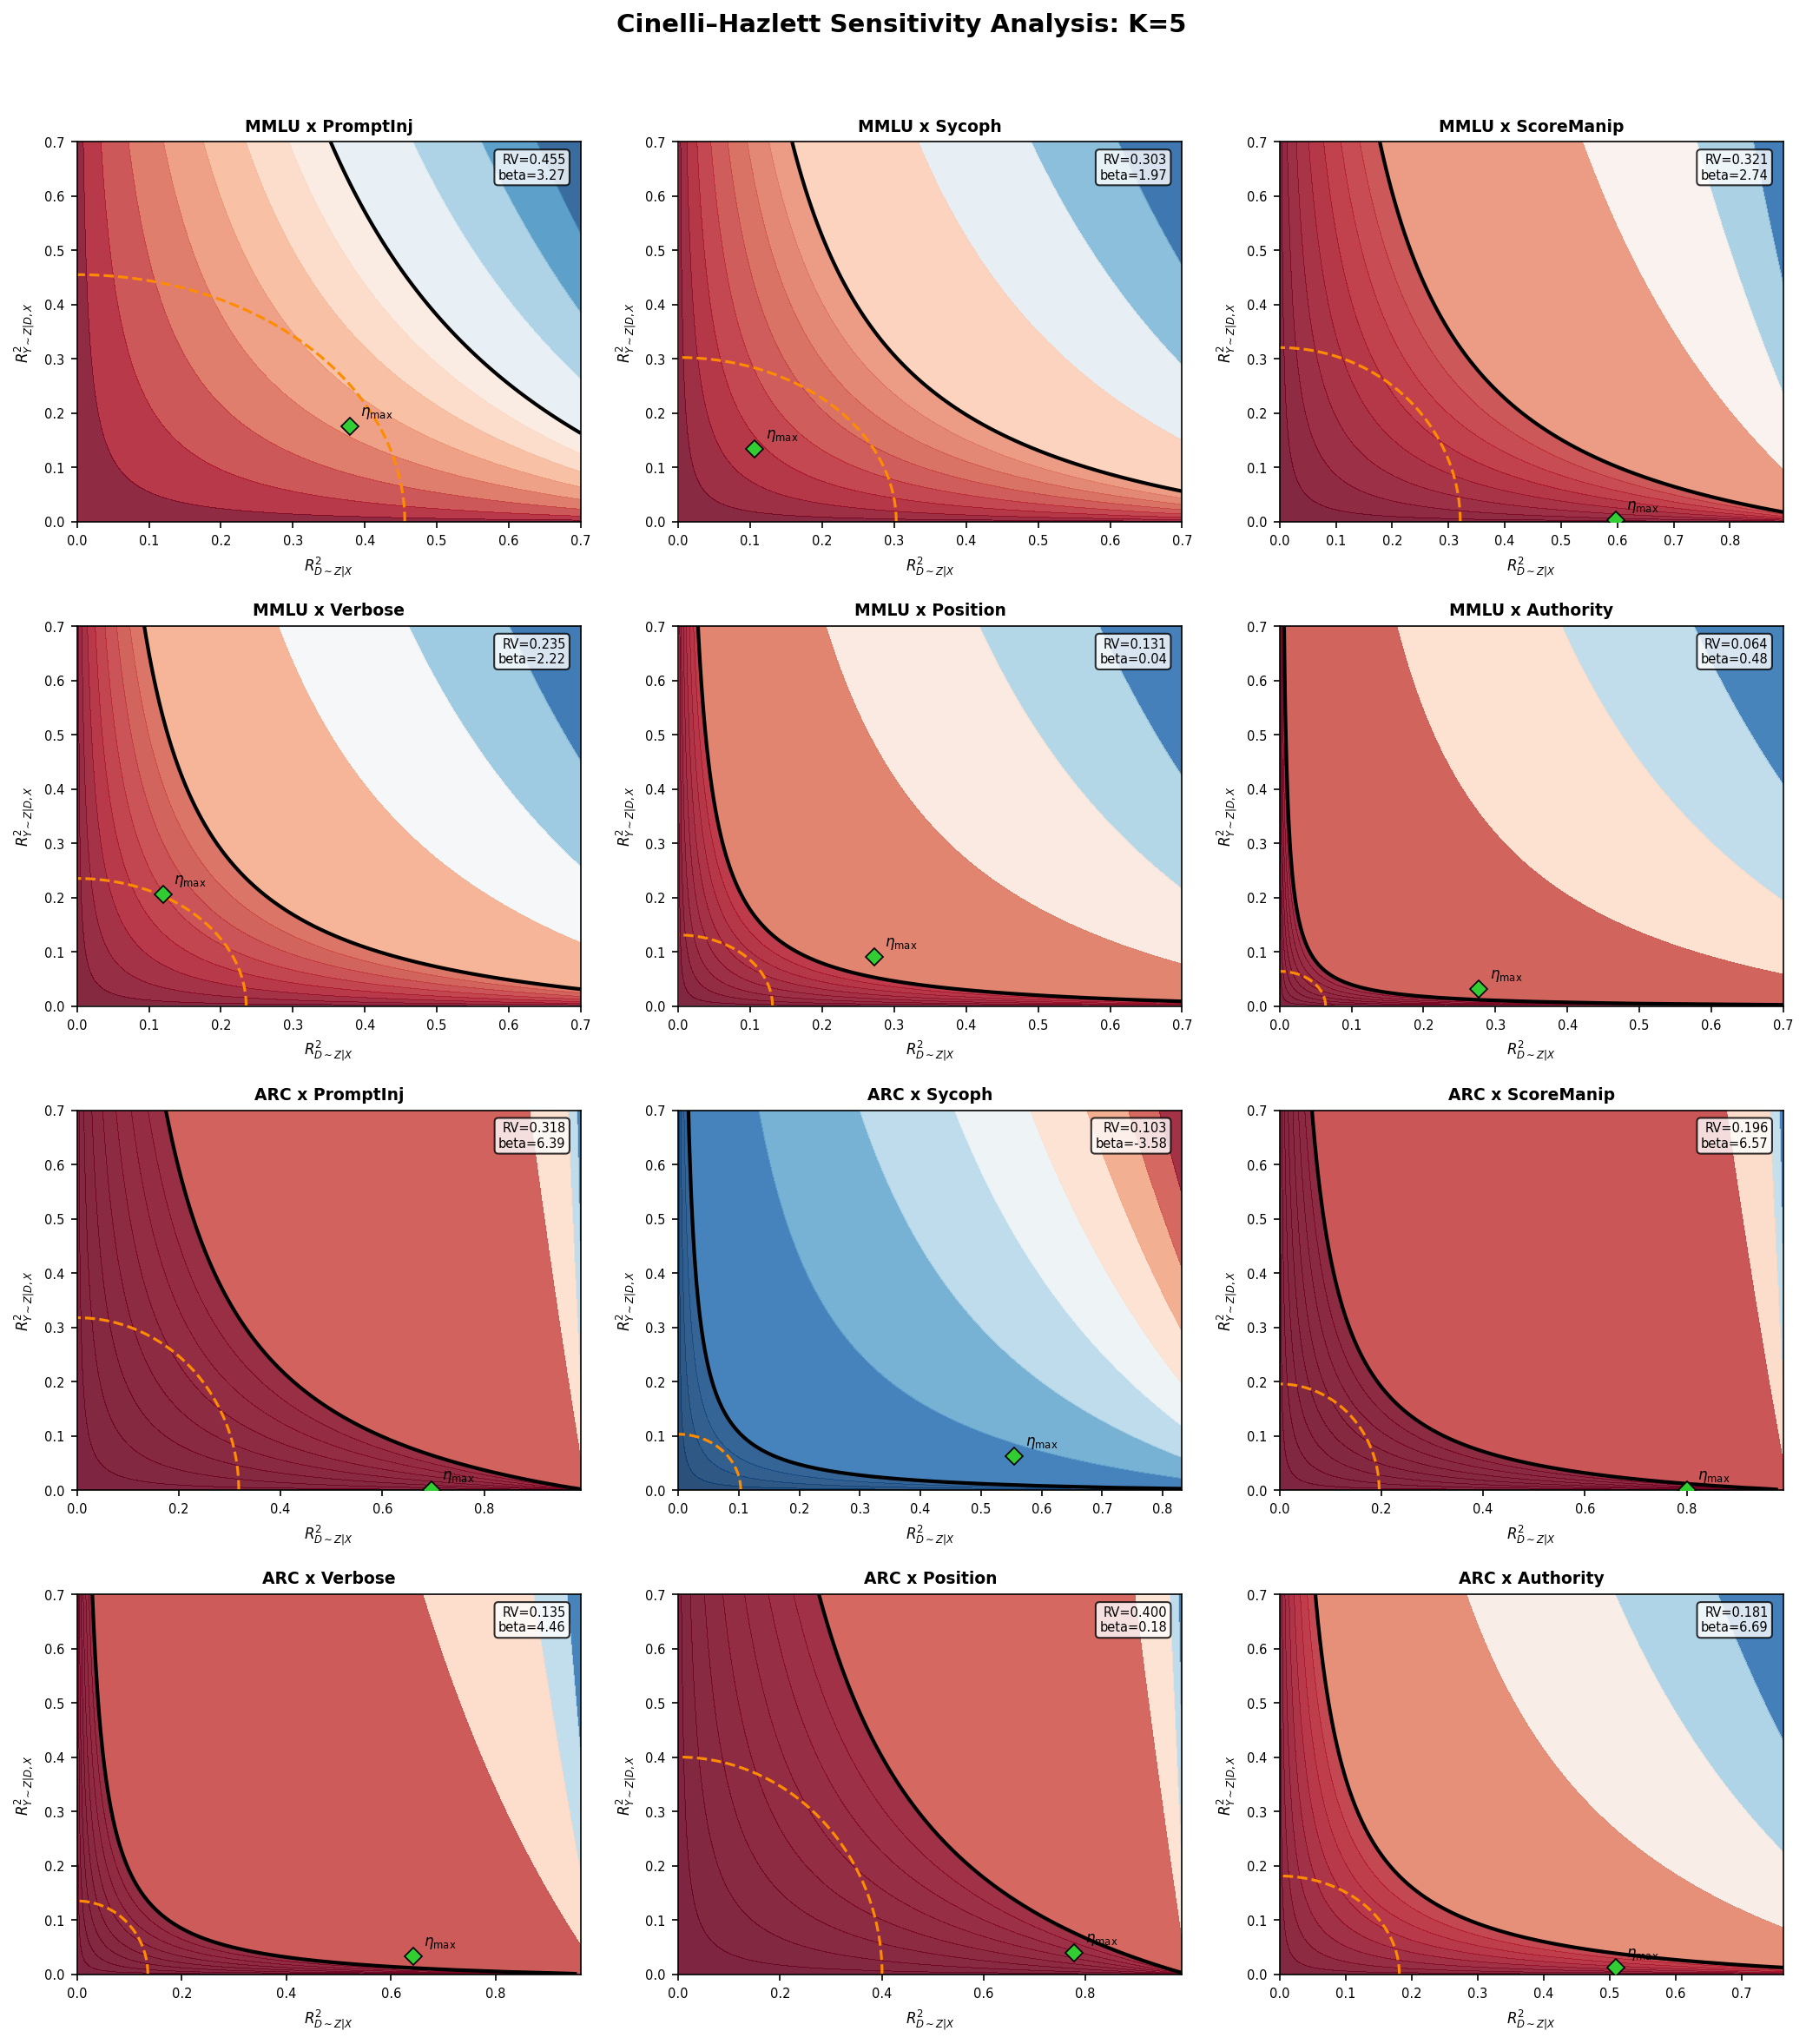
\includegraphics[width=\columnwidth]{figures/fig_sensitivity_contour_K5.png}
\caption{Cinelli--Hazlett sensitivity contour plot at $K{=}5$ (representative). $x$-axis: confounder's partial $R^2$ with treatment ($K_{\mathrm{eff}}$); $y$-axis: confounder's partial $R^2$ with outcome (ASR). Contour lines show the adjusted $K_{\mathrm{eff}}$ coefficient under hypothetical confounders of varying strength. The diamond marks the known $\eta_{\max}$ confound benchmark; conditions where the benchmark falls inside the zero-contour indicate that the $\eta_{\max}$ confound alone could explain away $K_{\mathrm{eff}}$'s effect.}
\label{fig:sensitivity_contour}
\end{figure}

\section{Cross-Benchmark Prediction Robustness}
\label{app:cross_benchmark}

To test whether the diversity--vulnerability association reflects structural panel properties rather than benchmark-specific artifacts, we use $K_{\mathrm{eff}}$ computed from one benchmark's pairwise MI to predict panel vulnerability on the other. Under wild cluster bootstrap (FDR $\alpha{=}0.05$), both directions achieve 17/18 sign-consistent conditions across $K \in \{3, 5, 7\}$ (5/6 at $K{=}3$, 6/6 at $K{\geq}5$). The sole exception in both directions is $K{=}3$ position bias, where all judges share similar ASR (${\sim}0.5$), leaving insufficient heterogeneity for $K_{\mathrm{eff}}$ to discriminate. Cross-benchmark $K_{\mathrm{eff}}$ correlations are $r{\approx}0.76$--$0.78$, indicating that $K_{\mathrm{eff}}$ primarily captures panel-level compositional structure rather than benchmark-specific judge interactions. While sign consistency is symmetric, cross-prediction $R^2$ is moderately asymmetric (ARC$\to$MMLU generally higher), suggesting that coefficients estimated from ARC's more constrained binary format generalize conservatively to MMLU's richer four-way choice distribution.

\section{Pool A Cinelli--Hazlett Sensitivity}
\label{app:sensitivity_poolA}

To test whether reducing the $K_{\mathrm{eff}}$--$\eta_{\max}$ collinearity strengthens $K_{\mathrm{eff}}$'s independent signal, we repeat the Cinelli--Hazlett analysis on the capability-matched Pool~A subsample (9 models, $r{=}0.50$, 84 panels at $K{=}3$, 126 at $K{=}5$). Table~\ref{tab:sensitivity_poolA} compares the full-pool results with Pool~A.

\begin{table}[h]
\centering
\small
\begin{tabular}{lccc}
\toprule
\textbf{Pool / $K$} & \textbf{RV $>$ $\eta$} & \textbf{Median RV} & \textbf{$K_{\mathrm{eff}}$ sig} \\
\midrule
Full / $K{=}3$ & 1/12 & 0.30 & 1/12 \\
Full / $K{=}5$ & 3/12 & 0.22 & 7/12 \\
Pool A / $K{=}3$ & 2/12 & 0.25 & --- \\
Pool A / $K{=}5$ & 10/12 & 0.32 & 9/12 \\
\bottomrule
\end{tabular}
\caption{Cinelli--Hazlett sensitivity comparison: full pool vs.\ capability-matched Pool~A. RV $>$ $\eta$: conditions where $K_{\mathrm{eff}}$'s robustness value exceeds the known $\eta_{\max}$ confound benchmark. Pool~A's reduced collinearity ($r{=}0.50$ vs.\ $0.81$ at $K{=}5$) increases the fraction of robust conditions from 1/12 to 2/12 at $K{=}3$ and from 3/12 to 10/12 at $K{=}5$, with the largest gains at $K{=}5$ where both benchmarks improve equally (ARC 5/6, MMLU 5/6).}
\label{tab:sensitivity_poolA}
\end{table}

At $K{=}5$, Pool~A RV exceeds the $\eta_{\max}$ confound in 10/12 conditions (ARC 5/6, MMLU 5/6; the two failures are both sycophancy). The improvement from full-pool 3/12 to Pool~A 10/12 demonstrates that reducing collinearity substantially separates $K_{\mathrm{eff}}$'s signal from capability variance, though full causal identification would require training-based diversity control.

\section{Epsilon Sensitivity Analysis}
\label{app:epsilon}

The log-log specification (Equation~\ref{eq:regression}) uses $\epsilon{=}10^{-6}$ to handle zero ASR values. We assess sensitivity by comparing coefficients across $\epsilon \in \{10^{-3}, 10^{-6}, 10^{-9}\}$. Zero ASR rates are low on MMLU ($<$1\% of panels across conditions) but can reach 38--40\% on ARC for authority bias and sycophancy at $K{=}7$. Coefficient magnitudes show moderate sensitivity to $\epsilon$ at $K{=}3$ (maximum $\Delta\beta_{\mathrm{std}} = 0.10$ between $\epsilon{=}10^{-6}$ and $\epsilon{=}10^{-9}$, with three conditions exhibiting $K_{\mathrm{eff}}$ sign changes), reflecting the influence of zero-ASR panels on the log transformation. At $K{=}5$, all $K_{\mathrm{eff}}$ coefficient directions are preserved across $\epsilon$ values (maximum $\Delta\beta_{\mathrm{std}} = 0.073$ between $\epsilon{=}10^{-6}$ and $\epsilon{=}10^{-9}$, all $p < 0.005$), confirming that the predictor shift finding is robust to this modeling choice. The fractional logit specification (\S\ref{sec:experiments}), which avoids the log+$\epsilon$ transformation entirely, provides 98.6\% directional concordance with the main OLS results (71/72 direction matches) (Appendix~\ref{app:robustness_checks}).

\section{Temperature Sensitivity Pilot}
\label{app:temperature}

We evaluate $K_{\mathrm{eff}}$ stability across decoding temperatures $t \in \{0.0, 0.3, 0.7, 1.0\}$ using a 3-model pilot (GPT-4.1-nano, Gemini-3.5-Flash, Claude-3-Haiku; 300 clean samples per benchmark, 3 repeats). The maximum $K_{\mathrm{eff}}$ variation across all four temperatures is $\Delta < 0.034$ (MMLU: 0.033, ARC: 0.027), confirming that decoding randomness does not meaningfully perturb pairwise MI structure. Clean $K_{\mathrm{eff}}$ computation is thus robust to temperature variation within the range used by standard API configurations.

\section{$K_{\mathrm{eff}}$ Distribution Statistics}
\label{app:keff_dist}

Table~\ref{tab:keff_dist} summarizes the distribution of $K_{\mathrm{eff}}$ across panel sizes.

\begin{table}[h]
\centering
\small
\begin{tabular}{rrccc}
\toprule
$\boldsymbol{K}$ & \textbf{Panels} & \textbf{Mean (SD)} & \textbf{Range} \\
\midrule
3 & 455     & 2.18 (0.30) & [1.47, 2.80] \\
5 & 3{,}003 & 3.35 (0.42) & [2.16, 4.30] \\
7 & 6{,}435 & 4.53 (0.47) & [2.97, 5.55] \\
\bottomrule
\end{tabular}
\caption{$K_{\mathrm{eff}}$ distribution across panel sizes. Mean $K_{\mathrm{eff}}$ increases approximately linearly with $K$ but remains below the theoretical maximum ($K_{\mathrm{eff}} = K$ for fully independent judges), reflecting non-zero inter-judge correlations.}
\label{tab:keff_dist}
\end{table}

$K_{\mathrm{eff}}$ exhibits sufficient variance at each $K$ for regression analysis (coefficient of variation 10--14\%), with no floor or ceiling effects that would compress the predictor range.

\section{Power Analysis Across Panel Sizes}
\label{app:power_analysis}

Table~\ref{tab:mde} reports minimum detectable effect sizes (MDE at 80\% power) under wild cluster bootstrap for each $K$. The sharp decrease in MDE from $K{=}3$ to $K{=}5$ (0.144 to 0.048) reflects both increased sample size ($455 \to 3{,}003$ panels) and more clusters per position. $K_{\mathrm{eff}}$'s partial significance at $K{=}3$ (4/12) is consistent with moderate power at this sample size; the 7/12 significance at $K{=}5$ is not type~I error inflation, as the design can detect effects as small as 0.048 SD.

\begin{table}[h]
\centering
\small
\begin{tabular}{rccc}
\toprule
$\boldsymbol{K}$ & \textbf{Panels} & \textbf{MDE ($\beta_{\mathrm{std}}$)} & \textbf{$K_{\mathrm{eff}}$ sig} \\
\midrule
3 & 455     & 0.144 & 4/12 \\
5 & 3{,}003 & 0.048 & 7/12 \\
7 & 6{,}435 & 0.036 & 8/12 \\
\bottomrule
\end{tabular}
\caption{Minimum detectable effect size (80\% power, 1{,}000 simulations, wild cluster bootstrap) by panel size. MDE decreases approximately as $1/\sqrt{N}$, confirming that $K{=}5$/$K{=}7$ significance reflects genuine effects rather than inflated type~I error.}
\label{tab:mde}
\end{table}

\section{Alternative Diversity Measures}
\label{app:alt_diversity}

We compare $K_{\mathrm{eff}}$ against three classical ensemble diversity measures using the same OLS specification (Equation~\ref{eq:regression}) with FDR correction across 12 conditions pooled over $K$ values.

\begin{table}[h]
\centering
\small
\begin{tabular}{lcccc}
\toprule
\textbf{Measure} & \textbf{Sig} & \textbf{Dir.} & \textbf{$|\bar{\beta}_{\mathrm{std}}|$} & $\boldsymbol{\rho}$ \textbf{w/} $\boldsymbol{K_{\mathrm{eff}}}$ \\
\midrule
$Q$-statistic    & 9/12  & 6+/3$-$ & 0.251 & 0.599 \\
Disagreement     & 11/12 & 11+/0$-$ & 0.481 & 0.934 \\
$\kappa$-diversity & 11/12 & 11+/0$-$ & 0.497 & 0.978 \\
\addlinespace
$K_{\mathrm{eff}}$ (ref.) & 12/12 & 12+/0$-$ & 0.430 & --- \\
\bottomrule
\end{tabular}
\caption{Comparison of diversity measures as predictors of panel ASR (OLS, FDR-corrected, 12 conditions pooled across $K$). Sig: FDR-significant conditions. $|\bar{\beta}_{\mathrm{std}}|$: mean absolute standardized coefficient. $\rho$: Pearson correlation with $K_{\mathrm{eff}}$.}
\label{tab:alt_diversity}
\end{table}

$K_{\mathrm{eff}}$ and $\kappa$-diversity \citep{kuncheva2003measures} are near-equivalent ($\rho{=}0.978$), with comparable significance counts (12/12 vs.\ 11/12) and effect sizes (0.430 vs.\ 0.497). Disagreement rate achieves similar predictive power ($\rho{=}0.934$, 11/12). The $Q$-statistic is the weakest predictor (9/12, $|\bar{\beta}_{\mathrm{std}}|{=}0.251$), consistent with its known insensitivity to the type of error correlation that is associated with panel vulnerability \citep{kuncheva2003measures}. $K_{\mathrm{eff}}$'s advantage over these alternatives is not predictive power but interpretability: it quantifies the number of effective independent channels in the panel, connecting directly to the information-theoretic foundation of panel aggregation (\S\ref{sec:experiments}).

\section{$\kappa$-Diversity Predictor Shift Comparison}
\label{app:kappa_regime}

To test whether the predictor shift (\S\ref{sec:cross_k}) is specific to $K_{\mathrm{eff}}$ or a generic property of diversity measures, we repeat the wild cluster bootstrap analysis replacing $K_{\mathrm{eff}}$ with $\kappa$-diversity ($1 - \bar{\kappa}$, where $\bar{\kappa}$ is the mean pairwise Cohen's $\kappa$ on clean winner labels; $\rho{=}0.978$ with $K_{\mathrm{eff}}$).

\begin{table}[h]
\centering
\small
\begin{tabular}{rcccc}
\toprule
& \multicolumn{2}{c}{\textbf{$K_{\mathrm{eff}}$}} & \multicolumn{2}{c}{\textbf{$\kappa$-diversity}} \\
\cmidrule(lr){2-3} \cmidrule(lr){4-5}
$\boldsymbol{K}$ & \textbf{div.\ sig} & $\boldsymbol{\eta_{\max}}$ \textbf{sig} & \textbf{div.\ sig} & $\boldsymbol{\eta_{\max}}$ \textbf{sig} \\
\midrule
3 & 4/12  & 3/12 & 8/12 & 1/12 \\
5 & 7/12 & 2/12 & 7/12 & 4/12 \\
7 & 8/12  & 1/12 & 6/12 & 1/12 \\
\bottomrule
\end{tabular}
\caption{Predictor shift comparison: $K_{\mathrm{eff}}$ vs.\ $\kappa$-diversity across panel sizes (wild cluster bootstrap, BH FDR $\alpha{=}0.05$). $K_{\mathrm{eff}}$ exhibits a clear shift ($4 \to 7 \to 8$); $\kappa$-diversity significance decreases monotonically ($8 \to 7 \to 6$), showing no predictor shift.}
\label{tab:kappa_regime}
\end{table}

$\kappa$-diversity is a stronger predictor than $K_{\mathrm{eff}}$ at $K{=}3$ (8/12 vs.\ 4/12), consistent with its larger mean effect size ($|\bar{\beta}_{\mathrm{std}}|{=}0.497$ vs.\ 0.430; Table~\ref{tab:alt_diversity}). However, $\kappa$-diversity shows no predictor shift: its significance \emph{decreases} from $K{=}3$ to $K{=}7$ ($8 \to 7 \to 6$), the opposite of $K_{\mathrm{eff}}$'s pattern ($4 \to 7 \to 8$). Furthermore, under $\kappa$-diversity, $\eta_{\max}$ retains significance at $K{=}5$ (4/12), whereas under $K_{\mathrm{eff}}$ it drops to 2/12. The predictor shift---co-determination at $K{=}3$ transitioning to diversity dominance at $K{\geq}5$---is thus specific to $K_{\mathrm{eff}}$'s MI-based formulation, which captures effective judge independence rather than pairwise label agreement.

\section{Gaussian Copula Assumption and $K_{\mathrm{eff}}$ Robustness}
\label{app:copula_gof}

$K_{\mathrm{eff}}$ admits a closed-form expression $K - \frac{1}{K}\sum_{i}\sum_{j \neq i} \rho_{ij}^2$ under the Gaussian copula, where $\exp(-2\,\mathrm{MI}(i,j)) = 1 - \rho_{ij}^2$ \citep{nelsen2006copulas}. We test whether this parametric assumption holds for judge pairs using the \citet{genest2008validity} Cram\'{e}r--von Mises goodness-of-fit test for Gaussian copulas.

\paragraph{GoF Results.} Across all $\binom{15}{2} = 105$ judge pairs, the Gaussian copula is rejected at $\alpha{=}0.05$ for 97--100\% of pairs (MMLU: 102/105, 97.1\%; ARC: 104/105, 99.0\%). The rejections are not marginal: median $p$-values are ${<}0.001$ on both benchmarks. This indicates that the pairwise dependence structure among LLM judges is substantially non-Gaussian, likely reflecting the discrete three-category nature of winner labels and the heavy tail structure of judge agreement patterns.

\paragraph{Ranking Robustness Despite Copula Rejection.} Despite the Gaussian copula being formally rejected, the closed-form $K_{\mathrm{eff}}$ (using $1 - \rho_{ij}^2$) and the plug-in MI $K_{\mathrm{eff}}$ (using $\exp(-2\,\widehat{\mathrm{MI}}(i,j))$ with Miller--Madow correction) produce highly concordant panel rankings within each $K$. Within-$K$ Spearman rank correlations are $\rho \approx 0.86$ ($K{=}3$: 0.862, $K{=}5$: 0.858, $K{=}7$: 0.867). The systematic level difference (plug-in $K_{\mathrm{eff}}$ mean 3.38 vs.\ closed-form 4.29, averaged across $K$) reflects the Miller--Madow bias correction increasing MI estimates, which compresses $\exp(-2\,\mathrm{MI})$ toward zero. This level shift does not affect regression results, which depend on ranking.

\paragraph{Implications.} $K_{\mathrm{eff}}$'s effectiveness as a predictor of panel vulnerability does not depend on the Gaussian copula being correct. The $\exp(-2\,\mathrm{MI})$ kernel provides a nonparametric, information-theoretic measure of pairwise alienation; the Gaussian copula merely offers a convenient closed-form approximation that preserves ranking fidelity. All regression analyses in the main text use the closed-form $K_{\mathrm{eff}}$; the plug-in MI version would yield equivalent conclusions for any analysis based on panel ordering.
